\chapter{Przegląd istniejących rozwiązań}
\section{Wstęp}
Zarówno technologia REST jak i RPC nie są czymś nowy w świecie wymiany informacji pomiędzy systemami informatycznymi. Na rynku istnieje wiele lepszych lub gorszych rozwiązań, które można użyć przy projektowaniu i budowie architektury mikroserwisowej. Rozdział ten ma na celu przybliżenie najpopularniejszych dostępnych w chwili tworzenia pracy.
\section{Rozwiązania oparte na technologii REST}
\subsection{Spark Java}
Powstała w roku 2014 biblioteka dedykowana językom Java oraz Kotlin. Założeniem autora było stworzenie technologii, która ułatwiałaby budowanie serwisów sieciowych bez zbędnego narzutu dodatkowych modułów tak jak ma to miejsce w rozwiązaniach typu Spring lub Jersey. W skład biblioteki wchodzą klasy odpowiedzialne za routing, ciasteczka, sesje, filtrowanie, obsługę błędów itp. Niewielkie rozmiary oraz podstawowa obsługa żądań REST sprawia, że idealnie nadaje się do tworzenia niewielkich serwisów, a wykorzystanie dobrodziejstw jakie przynosi ósme wydanie języka Java (funkcje lambda) pozwala pisać przejrzysty i kompaktowy kod.
\begin{lstlisting}[language=Java, caption=Przykład metody zwracającej tekst w Spark Java]
        import static spark.Spark.*;
        
        public class HelloWorld {
            public static void main(String[] args) {
                get("/hello", (req, res) -> "Hello World");
            } 
        }
        \end{lstlisting}
\subsection{Flask}
Python jest jednym z języków, który jest polecany do tworzenia mikroserwisów ze względu na minimalizm oraz olbrzymią dostępność  bibliotek wspomagających budowę API\@. Przeglądając dostępne rozwiązania dla tego języka najczęściej można natrafić na projekty wykorzystujące bibliotekę Flask, która posiada wbudowany router oraz pozwala pisać aplikacje składające się z modułów za pomocą obiektów zwanych Blueprints \cite{grinberg2018flask}. Ponadto mamy do dyspozycji cały wachlarz modułów odpowiedzialnych za zarządzenie sesją, logowanie, uwierzytelnianie oraz obsługę baz danych.
\begin{lstlisting}[language=Python, caption=Prosty model aplikacji z użyciem Flask]       
        from flask import Flask, jsonify


        # instantiate the app
        app = Flask(__name__)


        @app.route('/users/ping', methods=['GET'])
        def ping_pong():
            return jsonify({
                'status': 'success',
                'message': 'pong!'
            })
\end{lstlisting}
\subsection{HapiJS}
Postanie platformy nodejs, która zbudowana jest na podstawie silnika przeglądarki \textit{Chrome} zrewolucjonizowało świat aplikacji sieciowych. Pozwala on na budowanie asynchronicznego kodu serwerowego oraz aplikacji po stronie klienta w tym samym języku, czyli JavaScript. W chwili obecnej żadna inna technologia nie posiada tak wielu bibliotek oraz kompleksowych rozwiązań w swojej bazie. Jednym z popularniejszych jest stworzony w laboratoriach firmy Walmart HapiJS\@. W odróżnieniu od innych podobnych rozwiązań HapiJS dysponuje bogatą biblioteką wtyczek rozszerzających funkcjonalność\cite{brett2016getting}
\begin{center}
	\begin{lstlisting}[language=java, caption=Przykład uruchomienia serwera http w HapiJS]
'use strict';

const Hapi = require('hapi');

const server = Hapi.server({
  port: 3000,
  host: 'localhost'
});

server.route({
  method: 'GET',
  path: '/',
  handler: (request, h) => {
    return 'Hello, world!';
  }
});

server.route({
  method: 'GET',
  path: '/{name}',
  handler: (request, h) => {
    return 'Hello, ' + encodeURIComponent(request.params.name) + '!'
    }
});

const init = async () => {
  await server.start();
  console.log(`Server running at: ${server.info.uri}`);
};

process.on('unhandledRejection', (err) => {
  console.log(err);
  process.exit(1);
});

init();
    \end{lstlisting}
\end{center}
\subsection{ASP NET Core Web API}
W roku 2016 Microsoft zaprezentował platformę net core. Jest to odświeżony, w pełni modułowy zestaw bibliotek wraz z środowiskiem służącym do jego uruchomienia przygotowany do współpracy z systemami z rodziny Windows jak i dostępnymi na system Linux. Modułowa budowa pozwala na pobranie lub wykorzystanie tylko tych zależności jakie są wymagane do uruchomienia aplikacji. Są to między innymi biblioteki odpowiedzialne za obsługę baz danych, logowania zdarzeń, uwierzytelniania itp. Każda biblioteka jest dostępna w repozytorium NuGet skąd bardzo łatwo można ją dołączyć do projektu rozszerzając\cite{reynders2018modern} jego funkcjonalności.
\begin{lstlisting}[language=java, caption=Przykład definicji adresów URI dla metod http w kontrolerze]
[HttpGet]
public ActionResult<List<TodoItem>> GetAll()
{
    return _context.TodoItems.ToList();
}

[HttpGet("{id}", Name = "GetTodo")] 
public ActionResult<TodoItem> GetById(long id)
{
    var item = _context.TodoItems.Find(id);
    if (item == null)
    {
        return NotFound();
    }
    return item;
}
\end{lstlisting}
\section{Rozwiązania oparte na technologii RPC}
\subsection{CORBA}
CORBA (\textit{Common Object Request Broker Architecture}) jest ogólną specyfikacją zaproponowaną w roku 1991 przez stowarzyszenie OMG (\textit{Object Management Group}). Definiuje ona standard komunikacji w systemach rozproszonych oparty o paradygmat obiektowy. Do podstawowych wymagań\cite{bolton2002pure} systemów implementujących standard CORBA należą:
\begin{itemize}
	\item \textbf{Orientacja obiektowa}-wszystkie zdalne operacje są grupowane w interfejsach podobnie jak ma to miejsce w obiektowych językach programowania takich jak C++ lub Java. Instancją każdego interfejsu jest tzw. obiekt CORBA\@. Jeśli klient chce wywołać zdalnie musi znać dokładne informacje o zdalnym obiekcie. W tym wypadku, każdy obiekt powinien mieć zdefiniowaną referencje do obiektu.
	\item \textbf{Przezroczystość lokalizacji}-aby ułatwić używanie obiektów, każdy system zbudowany według specyfikacji CORBA musi zapewnić, że nie istotne w jakiej lokalizacji znajduje się obiekt. Dostęp do każdego obiektu musi zostać zapewniony bez względu, czy znajduje się on w przestrzeni adresowej tej samej aplikacji, czy też w innej. Obiekt może znajdować się nawet na innej maszynie zdalnej.
	\item \textbf{Neutralność względem języka programowania}-CORBA jest zaprojektowana w ten sposób, aby kod klienta i serwera mógł zostać utworzony w różnych językach oprogramowania. W tym wypadku całkowicie normalną jest sytuacja, gdyż klient napisany w języku Java wywołuje procedurę w obiekcie zaimplementowanym w języku Cobol.
	\item \textbf{Obsługa mostów}-organizacja OMG miała świadomość, że równolegle prowadzone są prace nad alternatywnymi systemami rozproszonymi takimi jak Microsoft DCOM lub RMI\@. W związku z tym zaistniała potrzeba integracji z tymi systemami. W konsekwencji powstało w późniejszym czasie wiele projektów umożliwiających łączenie ww. technologii z architekturą CORBA\@.
\end{itemize}
Interfejsy opisujące każdy obiekt definiuje się za pomocą specjalnie do tego stworzonego języka IDL (\textit{Interface Definition Language}). Jest to język czysto deklaratywny przeznaczony wyłącznie do definiowania struktury interfejsów. Na definicję obiektów przypadają używane typy danych, interfejsy oraz opisy operacji. Przestrzenie nazw (C++) oraz pakiety (Java) są definiowane za pomocą modułów. Każda sygnatura wywoływanej operacji (metody) zawiera:
\begin{itemize}
	\item identyfikator (nazwę),
	\item typ zwracanej wartości,
	\item parametry wywołania (typ oraz kierunek),
	\item wyjątki
\end{itemize}
\begin{lstlisting}[language={[CORBA]IDL}, caption=Przykład zapisu definicji interfejsu w języku IDL]
interface CustomerAccount {
    string get_name();
    long   get_account_no();
    boolean deposit_money(in float amount);
    boolean transfer_money(
        in float amount,
        in long  destination_account_no,
        out long confirmation_no
    );
};
\end{lstlisting}
Komunikacja pomiędzy klientem, a serwerem była oparta na zdalnym wywołaniu procedur. Początkowo wykorzystywano do tego specjalnie przygotowany protokół GIOP (\textit{General Inter-ORB Protocol}) niezależny od sieciowej warstwy transportowej, a od wersji 2.0 IIOP (\textit{Internet Inter-ORB Protocol}) oparty na warstwie transportowej TCP/IP\@. Budowa oraz zasady działania CORBA są bardzo złożone. Poniżej wymienione zostały podstawowe koncepcje opisujące architekturę technologii:
\begin{itemize}
	\item \textbf{Kompilatory IDL}-każdą aplikację CORBA rozpoczyna się od zdefiniowania określonych interfejsów z których zostanie wygenerowany kod dla klienta jak i serwera.
	\item \textbf{Mapowanie języków programowania}-specyfikacja języka IDL opisuje dokładnie każdy typ danych zdefiniowany w interfejsach wraz z mapowaniem do typów danych języków do których zostaną interfejsy skompilowane. W dokumentacji zawarty jest również sposób implementacji obiektów po stronie serwera.
	\item \textbf{Kod klienta oraz serwera}-wygenerowany kod klienta (\textit{stub})\\pozwala wywoływać zdalne operacje w obiektach CORBA w taki sposób jak ma to miejsce w obiektach lokalnych. Natomiast kod serwera (\textit{skeleton}) jest nadzbiorem kodu klienta pozwalając aplikacji serwerowej na implementację obiektu CORBA\@.
	\item \textbf{Referencja obiektu}-każdy klient odwołujący się do obiektu CORBA musi posiadać referencje do tego obiektu. W przypadku języków Java oraz C++ obiekt zawierający wywoływane metody sam w sobie posiada referencję. W momencie, gdy klient wywołuje zdalną operację zostaje przekierowany przez referencję do odpowiedniej lokalizacji. Następnie po stronie serwera wywołanie zostaje odebrane i przekierowane do odpowiedniego obiektu CORBA zaimplementowanego w kodzie serwera.
	\item \textbf{Adapter obiektu}-adapter jest pośrednikiem pomiędzy implementacją obiektu, a szyną ORB (\textit{Object Request Broker}). Odpowiada on za generowanie referencji do obiektów, wywołania metod oraz zapewnienie bezpieczeństwa w komunikacji. W wczesnych wersjach CORBA zdefiniowany był jako BOA (\textit{Basic Object Adapter}) jednak był on niedokładnie zdefiniowany co skutkowało brakiem kompatybilności pomiędzy różnymi implementacjami szyny ORB\@. W wersji 2.2 oraz późniejszych dodano adapter POA (\textit{Portable Object Adapter}) z uszczegółowioną specyfikacją oraz wieloma rozszerzeniami umożliwiając już w pełna przenośność.
	\item \textbf{Pośrednik Zleceń Obiektowych}-ORB jest zasadniczą częścią technologii CORBA\@. Jest to zbiór całego oprogramowania umożliwiającego komunikacje pomiędzy obiektami w sieci. Pośrednik zapewnia mechanizm lokalizowania oraz aktywowania zdalnych serwerów oraz uzyskuje referencję do obiektów w aplikacji. Ponadto odpowiada za komunikację do innego pośrednika.
\end{itemize}
CORBA pomimo bardzo bogatej funkcjonalności została wyparta przez inne technologie opisane w dalszej części niniejszej pracy. Duża złożoność implementacji, problemy z bezpieczeństwem oraz brak wersjonowania to główne powody zaniechania stosowania tej technologii w systemach budowanych po roku 2000. Ponadto CORBA całkowicie pomijała platformę .NET, która jest jedną z głównych stosowanych w oprogramowaniu korporacyjnym.

\subsection{Protokół XML-RPC}
W roku 1998 utworzono protokół XML-RPC, którego zadaniem była komunikacja w konfiguracji klient-serwer. Protokół ten jest kombinacją architektury RPC, języka znaczników XML oraz protokołu HTTP co powoduje, że do jego implementacji można użyć istniejącej infrastruktury sieciowej oraz dostępnych technologii przesyłania danych\cite{laurent2001programming}. XML-RPC jest technologią całkowicie niezależną od zastosowanej architektury oraz języka programowania umożliwiając w pełni działanie w systemach heterogenicznych. Zasada działania protokołu polega na synchronicznym przesyłaniu pakietów danych pomiędzy klientem, a serwerem w postaci żądań oraz odpowiedzi HTTP tak samo jak robią to przeglądarki internetowe z tą różnicą, że dane są reprezentowane w formacie XML\@. Bezstanowa natura protokołu HTTP sprawia, że protokół XML-RPC również posiada tą właściwość. Powoduje ona, że dwa identyczne wywołania zdalnej metody jedno po drugim są traktowane jako nie związane niczym zdarzenia, a żadna z wartości jakie przekazują nie jest nigdzie zapisywana. Poniżej został przedstawiony proces wywołania zdalnej procedury oraz odpowiedzi przez serwer:
\begin{enumerate}
	\item aplikacja za pomocą klienta XML-RPC wykonuje zdalne wywołanie metody \\ określając nazwę metody, parametry wywołania oraz adres serwera,
	\item klient XML-RPC umieszcza wszystkie przekazane dane w strukturze xml.
	      Aplikacja wysyła tak przygotowaną strukturę jako żądanie POST na wskazany adres serwera,
	\item serwer HTTP przyjmuje żądanie od klienta przekazując dane ze struktury XML do słuchacza XML-RPC,
	\item słuchacz parsuje odebrane dane i wywołuje odpowiednią metodę wraz z parametrami,
	\item wywołana metoda zwraca wynik operacji do procesu XML-RPC, który przetwarza je do struktury XML,
	\item serwer zwraca tak przygotowaną odpowiedź do klienta,
	\item klient XML-RPC parsuje wynik z struktury XML przekazując dane do aplikacji, która w dalszej kolejności kontynuuje ich przetwarzanie
\end{enumerate}
Serwer jak i klient mogą zamienić się miejscami, tylko ważne jest aby zachowany był podział na serwer-klient. Protokół XML-RPC definiuje reprezentację podstawowych typów danych przekazywanych w żądaniach oraz zwracanych w odpowiedzi:
\begin{table}[h]
	\caption{Podstawowe typy danych i ich reprezentacja w strukturze XML-RPC}
	\footnotesize
	\begin{center}
		\begin{tabular}{ |c|c| }
			\hline
			\textbf{Typ danych}       & \textbf{Znacznik XML}                                  \\
			\hline
			Liczby Całkowite          & <int>400</int>                                         \\
			\hline
			Liczby Zmiennoprzecinkowe & <double>2.0</double>                                   \\
			\hline
			Zmienne logiczne          & <boolean>1</boolean>                                   \\
			\hline
			Typy łańcuchowe           & <string>Hello, World!</string>                         \\
			\hline
			Data i czas               & <dateTime.iso8601>19030223T00:30:00</dateTime.iso8601> \\
			\hline
			Typ binarny               & <base64>UGF3ZcWCIFNham7Ds2c=</base64>                  \\
			\hline
		\end{tabular}
	\end{center}
\end{table}
\newpage
Za pomocą notacji xml można również zapisać bardziej skomplikowane typy danych jakimi są struktury oraz tablice składające się z typów prostych. Definicje struktur oraz tablic przedstawiają się następująco:
\begin{lstlisting}[language=XML, caption=Reprezentacja tablicy w XML-RPC]
<array> 
  <data> 
    <value> Some Value</value> 
      ...
    <value> Some Value </value> 
  </data> 
</array> 
\end{lstlisting}
\begin{lstlisting}[language=XML, caption=Reprezentacja struktury w XML-RPC]
<struct> 
  <member> 
    <name>Name-1</name> 
    <value>Value-1</value> 
  </member> 
    ... 
  <member> 
    <name>Name-n</name> 
    <value>Value-n</value> 
  </member> 
</struct> 
\end{lstlisting}
Każde żądanie XML-RPC składa się z nagłówka oraz danych właściwych przestawionych w notacji xml. W nagłówku podobnie jak w zwykłych żądaniu http znajdują się informacje o nazwie serwera, rodzaju wywoływanej metody, ścieżką wywoływanego skryptu oraz typu danych.
\begin{lstlisting}[language=XML, caption=Przykład żądania POST]
POST /rpchandlefunc HTTP/1.0  
User-Agent: MySystemXMLRPC/1.0  
Host: xmlrpc.server.com  
Content-Type: text/xml  
Content-Length: 165  

<?xml version="1.0"?>  
<methodCall> 
<methodName>getCapitalCity</methodName> 
<params> 
<param> 
<value><string>England</string></value> 
</param> 
</params> 
</methodCall>  
\end{lstlisting}
W przypadku odpowiedzi zwracany jest wynik wywołania metody lub wyjątek z błędem w przypadku nie powodzenia w postaci struktury nazwanej fault. Każdy błąd posiada swój kod z zakresu od -32768 do -32000. W nagłówku znajduje się kod odpowiedzi http, adres serwerem, który został przekazany jako parametr  User-Agent w żądaniu przez klienta. W języku Java protokół został rozszerzony dodatkowo o specjalny typ \textit{<nil/>} reprezentujący znany w javie null.

\begin{lstlisting}[language=XML, caption=Przykład odpowiedzi serwera]
HTTP/1.1 200 OK   
Date: Sun, 29 Apr 2001 12:08:58 GMT
Server: Apache/1.3.12 (Unix) Debian/GNU PHP/4.0.2  
Connection: close  
Content-Type: text/xml  
Content-length: 133  
 
<?xml version="1.0"?> 
<methodResponse> 
<params> 
<param> 
<value><string>Michigan</string></value> 
</param> 
</params> 
</methodResponse> 
\end{lstlisting}
\noindent
Pomimo wielu zalet protokół XML-RPC posiada również kilka znaczących wad, które sprawiają, że wykorzystanie go w komunikacji pomiędzy mikroserwisami nie będzie najbardziej optymalnym rozwiązaniem:
\begin{itemize}
	\item w związku z tym, że żądania oraz odpowiedzi są przekazywane w języku XML ich wielkość jest znacząca,
	\item protokół sam w sobie nie posiada ważnych mechanizmów zapewniających bezpieczeństwo,
	\item protokół http na którym bazuje XML-RPC nie jest wydajny,
	\item użytkownik nie może zdefiniować swoich typów, musi polegać na tych wbudowanych
\end{itemize}
\subsection{SOAP}
Rosnąca na początku XXI wieku popularność architektury SOA (\textit{Service Oriented Architecture}) spowodowała pojawienie się różnych rozwiązań opartych na modelu współpracujących ze sobą komponentów usługowych, komunikujących się za pomocą sieci Internet. Oprócz wspomnianych wcześniej technologii CORBA oraz DCOM pojawiło się również rozwiązanie o nazwie Web Services, które zdobyło bardzo dużą popularność. Każdego dnia miliony użytkowników na świecie korzysta z serwisów internetowych podczas zakupów w sklepach internetowych, zamawianiu biletów na środki komunikacji publicznej czy korzystając z komunikatora internetowego w telefonie komórkowym. Każdy komponent działający w technologii Web Service składa się z następujących części\cite{snell2002programming}:
\begin{itemize}
	\item Aplikacji przetwarzającej logikę biznesową. W tym miejscu może to być koszyk przechowujący zakupy w sklepie internetowym, moduł cenowy itp.,
	\item Service Listener-serwis sieciowy nasłuchujący, który odbiera przychodzące żądania klienta,
	\item  Service Proxy-serwis dekodujący przychodzące żądanie z serwisu nasłuchującego przekazujący dane do aplikacji serwerowej,
	\item Serwer aplikacji-serwer HTTP służący jako kontener na serwisy
\end{itemize}
\begin{figure}[ht]
	\caption{Ogólny zarys budowy typowej usługi sieciowej}
	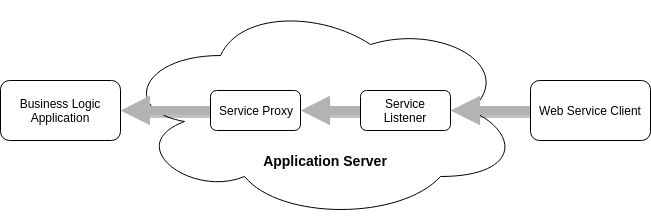
\includegraphics[width=\textwidth]{web_service}
	\centering
\end{figure}
\newpage
\noindent
Do najważniejszych rozwiązań wchodzących w skład technologii Web Services należą:
\begin{itemize}
	\item \textbf{SOAP (\textit{ Simple Object Access Protocol})}-protokół komunikacyjny służący do przekazywania zdalnych wywołań,
	\item \textbf{WSDL (\textit{Web Service Description Language})}-język oparty na XML służący do definiowania interfejsów usługi,
	\item \textbf{UDDI (\textit{Universal Description, Discovery, and Integration})}-rejestr wszystkich serwisów, które są dostępne zawierający ich metadane. Pobierając definicje z dokumentów WSDL służy do wyszukiwania udostępnionych usług, które mogą zainteresować potencjalnego konsumenta.
\end{itemize}
Protokół SOAP oparty na języku XML może korzystać z wielu dostępnych mechanizmów warstwy transportowej takich jak HTTP, HTTPS, SMTP lub JABBER\@. Wywoływanie usług następuje w dwóch trybach:
\begin{enumerate}
	\item RPC (\textit{Remote Procedure Call})-w tym trybie XML reprezentuje listę parametrów wraz z wartościami, która zostaje przekazana komponentowi,
	\item EDI (\textit{Electronic Document Interchange})-usługa otrzymuje tylko jeden parametr wywołania, którym jest cały dokument XML zawierający wszystkie dane składające się na encję biznesową.
\end{enumerate}
\par Komunikaty SOAP zbudowane są ze znaczników XML\@. Najwyżej w hierarchii znajduje się znacznik \textbf{<Envelope>} oznaczający początek całego komunikatu. W dalszej kolejności znajduje się opcjonalny \textbf{<Header>} zawierający informacje nagłówkowe. Znacznik \textbf{<Body>} skupia wszystkie informacje o żądaniu oraz odpowiedzi. Uzupełnieniem powyższej listy jest znacznik \textbf{<Fault>} w którym znajdują się ewentualne błędy z kodami oraz opisami, jakie mogły pojawić się podczas przetwarzania żądania.
\begin{lstlisting}[language=xslt, caption=Przykład żądania SOAP]
<?xml version="1.0"?>
<soap:Envelope xmlns:soap="http://www.w3.org/2001/12/soap-envelope"
 soap:encodingStyle="http://www.w3.org/2001/12/soap-encoding">
    <soap:Body xmlns:m="calculator">
      <m:multiply>
        <m:value_one>8</m:value_one>
        <m:value_two>5</m:value_two>
      </m:multiply>  
    </soap:Body>
</soap:Envelope> 
\end{lstlisting}
Powyższy listing przedstawia wywołanie metody \textit{multiply}, która należy do komponentu \textit{calculator}. Do wywołania metody są przekazane dwa parametry \textit{value\_one} oraz \textit{value\_two} z uzupełnionymi wartościami. W odpowiedzi serwer może zwrócić wynik tak jak przedstawia to listing poniżej.
\begin{lstlisting}[language=xml, caption=Odpowiedź SOAP serwera na żadanie klienta] 
<?xml version="1.0"?>
<soap:Envelope xmlns:soap="http://www.w3.org/2001/12/soap-envelope"
  soap:encodingStyle="http://www.w3.org/2001/12/soap-encoding">
  <soap:Body xmlns:m="demo">
    <m:multiplyRes>
      <m:result>40</m:result>
    </m:multiplyRes>
  </soap:Body>
</soap:Envelope> 
\end{lstlisting}
Wywołania usług zdalnych mogą przebiegać w sposób synchroniczny (protokół HTTP) lub asynchroniczny (JABBER, BEEP).
Technologia SOAP jest bardzo złożona jednak bardzo popularna w rozwiązaniach korporacyjnych z uwagi na rozbudowany opis serwisów w WSDL oraz wykorzystanie XML\@.
\subsection{Apache Thrift}
Apache Thrift jest jedną z najnowszych technologii opartych na protokole RPC\@. Rozwiązanie to zostało opracowane w firmie Facebook w roku 2006, gdzie wykorzystywano je do komunikacji pomiędzy setkami serwisów tworzących ten portal społecznościowy. Po roku zdecydowano się go przekazać fundacji Apache, gdzie stał się technologią open source. W dniu dzisiejszym wykorzystywany jest przy takich projektach jak Twitter, Pinterest lub Evernote. Podobnie jak wcześniej opisane technologie tak w tym przypadku wykorzystywany jest język IDL (\textit{Interface Definition Language}) specjalnie przygotowany do współpracy z Apache Thrift. \par Projekt powstał w czasie, gdy Facebook rozpoczął swoją ekspansję na cały świat. Inżynierowie pracujący w projektach pobocznych zauważyli, że dotychczasowe rozwiązania oparte na zestawie LAMP nie są wystarczające\cite{slee2007thrift}. Poszukiwania dostępnych rozwiązań nie przyniosły oczekiwanych efektów, gdyż na wielu płaszczyznach posiadały ograniczenia nie możliwe do zaakceptowania. W tym właśnie momencie podjęto decyzję o zaprojektowaniu od podstaw technologii, która nie tylko rozwiąże problemy z którymi nie poradziły sobie inne podobne projekty, ale również te nowe dopiero powstałe. Poniżej przedstawiono główne koncepcje Apache Thrift:
\begin{itemize}
  \item \textbf{Obsługa wielu typów danych}-oprócz podstawowych typów takich jak łańcuchy znaków lub liczby Thrift pozwala również definiować struktury, kolekcje (map, list, set), wyjątki oraz metody, które są w tym przypadku obiektami,
  \item \textbf{Warstwa transportu}-możliwość transmisji danych za pomocą różnych kanałów. Do dyspozycji zostają oddane gniazda sieciowe, protokół HTTP, systemy plików, obiekty w pamięci lub biblioteka zlib.
  \item \textbf{Warstwa protokołu}-Apache Thrift zapewnia mechanizmy do automatycznej serializacji oraz deserializacji danych w postaci tekstu, zapisu binarnego, protokołu JSON itp.\ wszystko zleży od kontekstu. 
\end{itemize}